\documentclass{eurobot_report}

\usepackage{graphicx}
\usepackage{minted}

\begin{document}


\chapter{Communication I2C}

Le protocole I2C va nous permettre de communiquer entre les différents modules du robots. Dans le protocole I2C il y à un \textit{maitre} et un ou plusieurs \textit{ésclaves}. Il est important de noter que dans le protocole I2C, c'est uniquement le maitre qui initie une communication avec un esclave. 

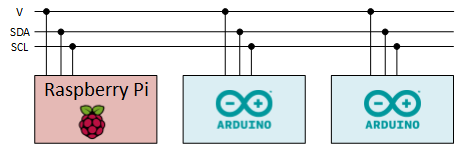
\includegraphics{assets/i2c.png}

Dans notre cas, la Raspberry Pi sera le maitre et les arduinos seront les ésclaves.

\section{Configuration Raspberry PI}
Sur la Raspberry PI, la pin \textbf{SDA} se trouve sur la pin 3 et la pin \textbf{SCL} se trouve sur la pin 5.

\begin{center}
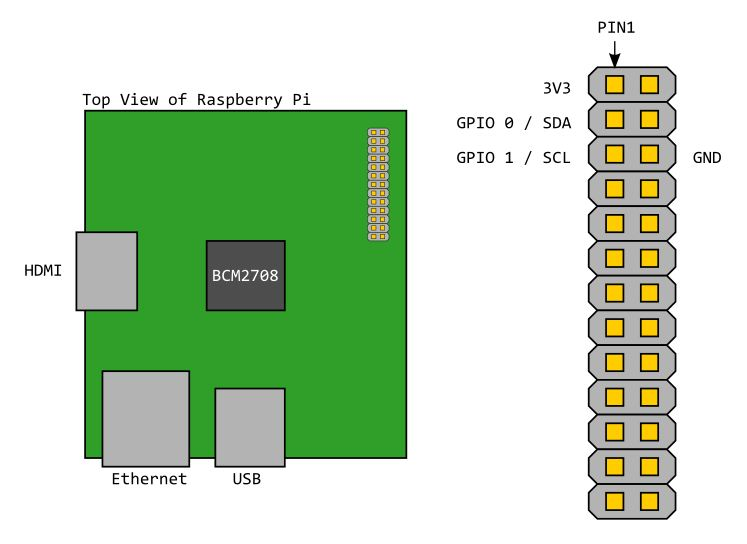
\includegraphics[width=12cm]{assets/rbp-i2c-pins}
\end{center}

Pour tester que les arduinos soient bien connectés, on peut utiliser la commande \textit{i2cdetect -y 1} qui va afficher les adresses des ésclaves connectés.

\begin{minted}{bash}
pi@raspberrypi:~ $ i2cdetect -y 1

     0  1  2  3  4  5  6  7  8  9  a  b  c  d  e  f
00:          -- 04 -- -- -- -- -- -- -- -- -- -- -- 
10: -- -- -- -- -- -- -- -- -- -- -- -- -- -- -- -- 
20: -- -- -- -- -- -- -- -- -- -- -- -- -- -- -- -- 
30: -- -- -- -- -- -- -- -- -- -- -- -- -- -- -- -- 
40: -- -- -- -- -- -- -- -- -- -- -- -- -- -- -- -- 
50: -- -- -- -- -- -- -- -- -- -- -- -- -- -- -- -- 
60: -- -- -- -- -- -- -- -- -- -- -- -- -- -- -- -- 
70: -- -- -- -- -- -- -- -- 
\end{minted}

On peut voir qu'il y à un ésclave connecté à l'adresse \textit{0x04}.

Pour employer la connexion I2C depuis le code Python, on utilise la librairie \textbf{smbus}. Celle-ci nous permet de lire et écrire des \textit{bytes} sur le bus I2C. Ci-dessous, vous pouvez voir un exemple d'un code Python qui envoie un nombre au hasard entre 0 et 180 sur le bus I2C à un ésclave connecté à l'adresse \textit{0x04} toute les 2 secondes. L'arduino qui reçoit ces données interprète ces nombres en angles pour commander un servo moteur.

\begin{minted}{python}
import smbus
import time
import random

bus = smbus.SMBus(1)
adr_arduino1 = 0x4
adr_arduino2 = 0x5
time.sleep(0.1)

while True:
    r = random.randrange(0, 180)
    bus.write_byte(adr_arduino1, r)
    print("Angle: ", r)
    time.sleep(2)
\end{minted}


\section{Configuration Arduino}
On utilise la librairie \textit{Wire.h} pour utiliser la communication I2C au niveau de l'arduino. Pour communiquer avec la raspberry, il faut correspondre l'adresse avec celle présente dans le code python de la raspberry. Ensuite dans la fonction \textit{setup}, configurer la librairie \textit{Wire.h} avec les fonctions \textit{begin(address)}, \textit{onReceive(fonction de réception)} et \textit{onRequest(fonction d'envoi)}. 

Dans un 2ème temps, il faut configurer les fonctions de réception et d'envoi. Pour recevoir une données par I2C avec la librairie \textit{Wire.h}, il suffit d'utiliser la fonction \textit{read()}. Pour envoyer une donnée, il suffit d'utiliser la fonction \textit{write(donnée)}. 

Dans l'exemple ci-dessous nous utilisons un servo-moteur avec les données envoyées par la raspberry (un angle).
\begin{minted}{arduino}
#include <Wire.h>
#include <Servo.h>

#define SLAVE_ADDRESS 0x12
int dataReceived = 0;
Servo monservo;

void setup() {
    Serial.begin(9600);
    Wire.begin(SLAVE_ADDRESS);
    Wire.onReceive(receiveData);
    Wire.onRequest(sendData);
}

void loop() {
    delay(100);
}

void receiveData(int byteCount){
    while(Wire.available()) {
        dataReceived = Wire.read();
        Serial.print("Donnee recue : ");
        monservo.write(dataReceived);
        Serial.println(dataReceived);
    }
}

void sendData(){
    int envoi = dataReceived + 1;
    Wire.write(envoi);
}
\end{minted}


\section{Structurer le code}
Dans le code de la Raspberry PI, qui gère le tout, on peut construire une classe par module qui crée une abstraction au dessus des communications I2C. Pour l'exemple du servo moteur, on pourrait avoir une classe \mintinline{python}|class Servo| qui fournit une méthode \mintinline{python}|def set_angle(angle)|. Cette méthode s'occuperait de la communication I2C avec l'arduino, ce qui produit une belle abstraction.

\section{Sources externes}
\href{http://www.pihomeserver.fr/2013/08/13/raspberry-pi-home-server-arduino-lier-les-deux-via-bus-i2c/}{I2C communication between Raspberry and Arduino}

\textbf{Smbus}(documentation library python to communicate i2c):
\begin{itemize}
\item \href{https://www.mjmwired.net/kernel/Documentation/i2c/smbus-protocol}{Functions details}
\item \href{http://wiki.erazor-zone.de/wiki:linux:python:smbus:doc}{Resume functions}
\end{itemize}


\end{document} 